\documentclass[journal,12pt,twocolumn]{IEEEtran}
%
\usepackage{setspace}
\usepackage{gensymb}
%\doublespacing
\singlespacing

\usepackage{graphicx}
\usepackage[cmex10]{amsmath}
\usepackage{amsmath,amsthm}
\usepackage{mathrsfs}
\usepackage{txfonts}
\usepackage{stfloats}
\usepackage{bm}
\usepackage{cite}
\usepackage{cases}
\usepackage{subfig}

\usepackage{longtable}
\usepackage{multirow}
\usepackage{commath}
\usepackage{enumitem}
\usepackage{mathtools}
\usepackage{steinmetz}
\usepackage{tikz}
\usepackage{circuitikz}
\usepackage{verbatim}
\usepackage{tfrupee}
\usepackage[breaklinks=true]{hyperref}

\usepackage{tkz-euclide}

\usetikzlibrary{calc,math}
\usepackage{listings}
    \usepackage{color}                                            
    \usepackage{array}                                            
    \usepackage{longtable}                                        
    \usepackage{calc}                                             
    \usepackage{multirow}                                         
    \usepackage{hhline}                                           
    \usepackage{ifthen}                                           
    \usepackage{lscape}     
\usepackage{multicol}
\usepackage{chngcntr}

\DeclareMathOperator*{\Res}{Res}

\renewcommand\thesection{\arabic{section}}
\renewcommand\thesubsection{\thesection.\arabic{subsection}}
\renewcommand\thesubsubsection{\thesubsection.\arabic{subsubsection}}

\renewcommand\thesectiondis{\arabic{section}}
\renewcommand\thesubsectiondis{\thesectiondis.\arabic{subsection}}
\renewcommand\thesubsubsectiondis{\thesubsectiondis.\arabic{subsubsection}}

\hyphenation{op-tical net-works semi-conduc-tor}
\def\inputGnumericTable{}                                 

\lstset{
%language=C,
frame=single, 
breaklines=true,
columns=fullflexible
}
\lstset{
%language=TeX,
frame=single, 
breaklines=true
}

\begin{document}

\newtheorem{theorem}{Theorem}[section]
\newtheorem{problem}{Problem}
\newtheorem{proposition}{Proposition}[section]
\newtheorem{lemma}{Lemma}[section]
\newtheorem{corollary}[theorem]{Corollary}
\newtheorem{example}{Example}[section]
\newtheorem{definition}[problem]{Definition}

\newcommand{\BEQA}{\begin{eqnarray}}
\newcommand{\EEQA}{\end{eqnarray}}
\newcommand{\define}{\stackrel{\triangle}{=}}
\bibliographystyle{IEEEtran}
\providecommand{\mbf}{\mathbf}
\providecommand{\pr}[1]{\ensuremath{\Pr\left(#1\right)}}
\providecommand{\qfunc}[1]{\ensuremath{Q\left(#1\right)}}
\providecommand{\sbrak}[1]{\ensuremath{{}\left[#1\right]}}
\providecommand{\lsbrak}[1]{\ensuremath{{}\left[#1\right.}}
\providecommand{\rsbrak}[1]{\ensuremath{{}\left.#1\right]}}
\providecommand{\brak}[1]{\ensuremath{\left(#1\right)}}
\providecommand{\lbrak}[1]{\ensuremath{\left(#1\right.}}
\providecommand{\rbrak}[1]{\ensuremath{\left.#1\right)}}
\providecommand{\cbrak}[1]{\ensuremath{\left\{#1\right\}}}
\providecommand{\lcbrak}[1]{\ensuremath{\left\{#1\right.}}
\providecommand{\rcbrak}[1]{\ensuremath{\left.#1\right\}}}
\theoremstyle{remark}
\newtheorem{rem}{Remark}
\newcommand{\sgn}{\mathop{\mathrm{sgn}}}
\providecommand{\abs}[1]{\(\left\vert#1\right\vert\)}
\providecommand{\res}[1]{\Res\displaylimits_{#1}} 
\providecommand{\norm}[1]{\(\left\lVert#1\right\rVert\)}
%\providecommand{\norm}[1]{\lVert#1\rVert}
\providecommand{\mtx}[1]{\mathbf{#1}}
\providecommand{\mean}[1]{E\(\left[ #1 \right]\)}
\providecommand{\fourier}{\overset{\mathcal{F}}{ \rightleftharpoons}}
%\providecommand{\hilbert}{\overset{\mathcal{H}}{ \rightleftharpoons}}
\providecommand{\system}{\overset{\mathcal{H}}{ \longleftrightarrow}}
	%\newcommand{\solution}[2]{\textbf{Solution:}{#1}}
\newcommand{\solution}{\noindent \textbf{Solution: }}
\newcommand{\cosec}{\,\text{cosec}\,}
\providecommand{\dec}[2]{\ensuremath{\overset{#1}{\underset{#2}{\gtrless}}}}
\newcommand{\myvec}[1]{\ensuremath{\begin{pmatrix}#1\end{pmatrix}}}
\newcommand{\mydet}[1]{\ensuremath{\begin{vmatrix}#1\end{vmatrix}}}
%\numberwithin{equation}{section}
\numberwithin{equation}{subsection}
%\numberwithin{problem}{section}
%\numberwithin{definition}{section}
\makeatletter
\@addtoreset{figure}{problem}
\makeatother
\let\StandardTheFigure\thefigure
\let\vec\mathbf
%\renewcommand{\thefigure}{\theproblem.\arabic{figure}}
\renewcommand{\thefigure}{\theproblem}
%\setlist[enumerate,1]{before=\renewcommand\theequation{\theenumi.\arabic{equation}}
%\counterwithin{equation}{enumi}
%\renewcommand{\theequation}{\arabic{subsection}.\arabic{equation}}
\def\putbox#1#2#3{\makebox[0in][l]{\makebox[#1][l]{}\raisebox{\baselineskip}[0in][0in]{\raisebox{#2}[0in][0in]{#3}}}}
     \def\rightbox#1{\makebox[0in][r]{#1}}
     \def\centbox#1{\makebox[0in]{#1}}
     \def\topbox#1{\raisebox{-\baselineskip}[0in][0in]{#1}}
     \def\midbox#1{\raisebox{-0.5\baselineskip}[0in][0in]{#1}}
\vspace{3cm}
\title{Assignment 2}
\author{Vishal Ashok}
\maketitle
\newpage
%\tableofcontents
\bigskip
\renewcommand{\thefigure}{\theenumi}
\renewcommand{\thetable}{\theenumi}
\begin{abstract}
This document explains how to trace a curve given its equation.
\end{abstract}
Download Python code from 
%
\begin{lstlisting}
https://github.com/vishalashok98/AI5106/tree/main/Assignment_1
\end{lstlisting}
%
Download the latex-tikz codes from 
%
\begin{lstlisting}
https://github.com/vishalashok98/AI5106/tree/main/Assignment_1
\end{lstlisting}
%

\section{Problem}

Trace the curve
\begin{align}
35x^2+30y^2+32x-108y-12xy+59=0 \label{given_curve_eq}
\end{align}


\section{Explanation}

The general equation of second degree is given by
\begin{align}
ax^2+2bxy+cy^2+2dx+2ey+f=0 \label{gen_quad_eqn}
\end{align}
and can be expressed as
\begin{align}
\vec{x}^T\vec{V}\vec{x}+2\vec{u}^T\vec{x}+f=0 \label{conic_quad_eqn}
\end{align}
where
\begin{align}
\vec{V} &= \vec{V}^T = \myvec{a & b \\ b & c}
\\
\vec{u}^T &= \myvec{d & e}
\end{align}

\section{Solution}


Comparing \eqref{given_curve_eq} with \eqref{gen_quad_eqn}, we get
\begin{align}
\vec{V} &= \myvec{35  & -6 \\ -6 & 30}
\\
\vec{u}^T &= \myvec{16 & -54}
\end{align}
If $\abs{\vec{V}} > 0$, then \eqref{conic_quad_eqn} is an ellipse. 
\begin{align}
\abs{V} = \begin{vmatrix}{35  & -6 \\ -6 & 30} \end{vmatrix}= 1014 > 0
\end{align}

\eqref{conic_quad_eqn} can be expressed as
\begin{align}
\label{conic_simp_temp_nonparab_eq}
\vec{y}^T\vec{D}\vec{y} &=  \vec{u}^T\vec{V}^{-1}\vec{u} -f  &  \abs{V} &\ne 0
\\
\vec{y}^T\vec{D}\vec{y} &=  -\eta\myvec{1 & 0}\vec{y}   & \abs{V} &= 0
\label{conic_simp_temp_parab_eq}
\end{align}
with center as 
\begin{align}
    \vec{c} &= - \vec{V}^{-1}\vec{u} & \abs{V} &\ne 0
\end{align}
Calculating the center for given curve we get,
\begin{align}
    \vec{c} &= - \frac{1}{\abs{35*30 - 6*6}}\myvec{35  & 6 \\ 6 & 30}\myvec{16 \\ -54} \\
    &= \frac{1}{1014}\myvec{236 \\ -1524} \\
    &= \myvec{\frac{118}{507}  \\\frac{254}{169}}
\end{align}

For 
\begin{align} 
\abs{\vec{V}} > 0, \quad \text{or, } \lambda_1 > 0, \lambda_2 > 0 
\end{align} 
\eqref{conic_simp_temp_nonparab_eq} becomes 
\begin{align} \lambda_1y_1^2 +\lambda_2y_1^2 = 
\vec{u}^T\vec{V}^{-1}\vec{u} -f 
\end{align} 
which is the equation of an ellipse with major and minor axes 
parameters
\begin{align} 
\sqrt{\frac{\lambda_1}{\vec{u}^T\vec{V}^{-1}\vec{u} -f}}, 
\sqrt{\frac{\lambda_2}{\vec{u}^T\vec{V}^{-1}\vec{u} -f}} \label{axes_eq}
\end{align}
The characteristic equation of $\vec{V}$ is obtained by evaluating the determinant
\begin{align}
\mydet{\lambda \vec{I}-\vec{V}} = \mydet{\lambda -35 & 6 \\ 6 & \lambda -30} &= 0
\\
\implies \lambda^2 - 65\lambda + 1014 &= 0
\label{ellipse_char_eq}
\end{align}
The eigenvalues are the roots of \eqref{ellipse_char_eq} given by
\begin{align}
\lambda_1 = 39, \lambda_2 = 26
\end{align}


Calculating the major and minor axes lengths using \eqref{axes_eq}, we get
\begin{align}
\vec{u}^T\vec{V}^{-1}\vec{u} &= \nonumber \\
&= \myvec{16 -54}\frac{1}{1014}\myvec{35 & 6 \\ 6 & 30 }\myvec{16 \\ -54} \nonumber \\
&= \frac{1}{1014}\myvec{16 & -54}\myvec{236 \\ -1524} \nonumber \\
&= \frac{43036}{507} \nonumber \\
\vec{u}^T\vec{V}^{-1}\vec{u} -f &= \frac{43036}{507} - 59 = \frac{13123}{507} \\
\sqrt{\frac{\vec{u}^T\vec{V}^{-1}\vec{u} -f}{\lambda_1}} &= \sqrt{\frac{13123}{19773}} = \frac{814}{1000} \\
\sqrt{\frac{\vec{u}^T\vec{V}^{-1}\vec{u} -f}{\lambda_2}} &= \sqrt{\frac{13123}{13182}} = \frac{997}{1000}
\end{align}


\begin{figure}[!ht]
\centering
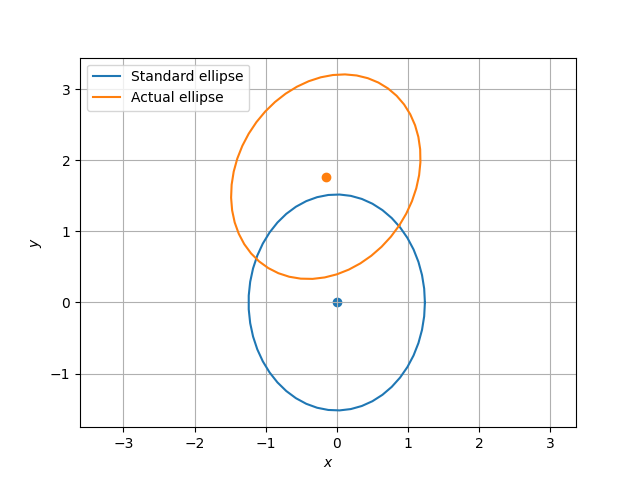
\includegraphics[width=\columnwidth]{LA Assignment/Figure_2.png}
\caption{Ellipse with center (\frac{118}{507} \frac{254}{169}) and having the axes lengths as \frac{814}{1000} and \frac{997}{1000}}
\label{Fig:Circle}
\end{figure}

\end{document}
